%%%%%%%%%%%%%%%%%%%%%%%%%%%%%%%%%%%%%%%%%
% Classic Lined Title Page
% LaTeX Template
% Version 1.0 (27/12/12)
%
% This template has been downloaded from:
% http://www.LaTeXTemplates.com
%
% Original author:
% Peter Wilson (herries.press@earthlink.net)
%
% License:
% CC BY-NC-SA 3.0 (http://creativecommons.org/licenses/by-nc-sa/3.0/)
%
% Instructions for using this template:
% This title page compiles as is. If you wish to include this title page in
% another document, you will need to copy everything before
% \begin{document} into the preamble of your document. The title page is
% then included using \titleAT within your document.
%
%%%%%%%%%%%%%%%%%%%%%%%%%%%%%%%%%%%%%%%%%

%----------------------------------------------------------------------------------------
%	PACKAGES AND OTHER DOCUMENT CONFIGURATIONS
%----------------------------------------------------------------------------------------



\documentclass[a4paper]{article}

\usepackage[utf8]{inputenc}
\usepackage{hyperref}
\usepackage{titlesec}
\usepackage{amssymb,amsmath}
\usepackage[italian]{babel}
\usepackage[titles]{tocloft}
\usepackage{appendix}
\hypersetup{%
    pdfborder = {0 0 0}
}
\usepackage{graphicx}
\usepackage[svgnames]{xcolor} % Required to specify font color
\usepackage{eurosym}

\newcommand*{\plogo}{\fbox{$\mathcal{PL}$}} % Generic publisher logo
\usepackage{listings}
\usepackage{fancyhdr}
\usepackage{lastpage}
\usepackage{ragged2e}
\usepackage{listingsutf8}
\usepackage{mathtools}\usepackage{chngcntr}
\usepackage{float}
\usepackage{longtable}

%----------------------------------------------------------------------------------------
%	TITLE PAGE
%----------------------------------------------------------------------------------------

\newcommand*{\titleAT}{\begingroup % Create the command for including the title page in the document
\newlength{\drop} % Command for generating a specific amount of whitespace
\drop=0.1\textheight % Define the command as 10% of the total text height

\rule{\textwidth}{1pt}\par % Thick horizontal line
\vspace{2pt}\vspace{-\baselineskip} % Whitespace between lines
\rule{\textwidth}{0.4pt}\par % Thin horizontal line

\vspace{\drop} % Whitespace between the top lines and title
\begin{center} % Center all text
\textcolor{Black}{ % Red font color
{\Huge Progetto}\\[0.5\baselineskip] % Title line 1
{\Large di}\\[0.75\baselineskip] % Title line 2
{\Huge Tecnologie Web}} % Title line 3
\\[2\baselineskip]
{\Large 21 giugno 2016}

\vspace{0.25\drop} % Whitespace between the title and short horizontal line
\rule{1\textwidth}{0.4pt}\par % Short horizontal line under the title
\vspace{\drop} % Whitespace between the thin horizontal line and the author name

\begin{tabular}{l | r}

\hline
\textbf{URL} & http://www.auxils.it \\
\hline
\textbf{Autore} & Gabriele Marcomin \\
\hline
\textbf{Distribuzione} & Prof.ssa Ombretta Gaggi \\
\hline
\textbf{Email referente} & gabriele.marcomin@gmail.com \\
\hline
\end{tabular}

\end{center}

\vfill % Whitespace between the author name and publisher text
\vfill
{\large Università degli studi di Padova}



%\rule{\textwidth}{0.4pt}\par % Thin horizontal line
%\vspace{2pt}\vspace{-\baselineskip} % Whitespace between lines
%\rule{\textwidth}{1pt}\par % Thick horizontal line

\endgroup}

\titleformat{\chapter}[display]
{}{\hfill\rule{.7\textwidth}{3pt}}{2pt}
{\hspace*{.3\textwidth}\huge\bfseries}[\addvspace{1pt}]
\titleformat{name=\chapter,numberless}[display]
{}{\hfill\rule{.7\textwidth}{3pt}}{2pt}
{\hspace*{.3\textwidth}\huge\bfseries}[\addvspace{1pt}]

\renewcommand*\contentsname{Indice}

\newcommand{\glossario}[1]{\textit{#1\ped{G}}}

\lstset{frame=shadowbox,
  language=c++,
  aboveskip=10mm,
  belowskip=10mm,
  showstringspaces=false,
  columns=flexible,
  basicstyle={\small\ttfamily},
  numbers=none,
  numberstyle=\tiny\color{gray},
  keywordstyle=\color{blue},
  commentstyle=\color{gray},
  stringstyle=\color{red},
  breaklines=true,
  breakatwhitespace=true
  tabsize=1
}
\lstset{inputencoding=utf8/latin1}

\renewcommand{\lstlistingname}{Listato}
\renewcommand{\footrulewidth}{0.4pt}

\newcommand{\changefont}{%
    \fontsize{5}{7}\selectfont
}

\def\arraystretch{2}

\DeclarePairedDelimiter\ceil{\lceil}{\rceil}
\DeclarePairedDelimiter\floor{\lfloor}{\rfloor}

%----------------------------------------------------------------------------------------
%	CONSTANTS
%----------------------------------------------------------------------------------------

\newcommand{\authorName}{Gabriele Marcomin}

%----------------------------------------------------------------------------------------
%	DOCUMENT HEADER
%----------------------------------------------------------------------------------------

\begin{document}
\titleAT % This command includes the title page
\pagestyle{empty}
\newpage
\tableofcontents
\newpage
\listoffigures
\clearpage

%----------------------------------------------------------------------------------------
%	HEADER FORMAT
%----------------------------------------------------------------------------------------

\fancyhf{}
\fancyhead[RE]{\small\scshape\nouppercase{\leftmark}}
\fancyhead[LO]{\small\scshape\nouppercase{\rightmark}}
\fancyhead[LE,RO]{\small\thepage}
\lhead{\rightmark}
\rhead{Progetto di Tecnologie web}
\rfoot{\thepage/\pageref{LastPage}}
\lfoot{\authorName}




%----------------------------------------------------------------------------------------
%	CONTENT
%----------------------------------------------------------------------------------------

\raggedright
\pagestyle{fancy}

\section{Abstract}
La seguente relazione ha il compito di illustrare le fasi di progettazione, realizzazione e test del progetto da me svolto.
Il progetto consiste nella realizzazione di un sito che sia al contempo usabile ed accessibile da tutte le categorie di utenti sia che siano disabili, sia che siano normodotati.\\
Il sito da me realizzato è un sito di tipo blog intitolato Auxils.it, il quale tratta notizie riguardanti il mondo open source.\\ 
Il sito dovrà possedere le seguenti caratteristiche:

\begin{enumerate}
  \item il sito web deve essere realizzato con lo standard XHTML Strict;
  \item il layout deve essere realizzato con CSS puri;
  \item il sito web deve rispettare la completa separazione tra contenuto, presentazione e comportamento
  \item il sito web deve essere accessibile a tutte le categorie di utenti interessate;
  \item il sito web deve organizzare i propri contenuti in modo da poter essere facilmente reperiti da qualsiasi utente;
  \item le funzionalità introdotte attraverso l'uso di script Javascript devono essere disponibili in altri modi anche nel caso in cui Javascript sia stato disattivato dall'utente.
  \item il sito web deve contenere pagine che utilizzino gli script per collezionare e pubblicare dati inseriti dagli utenti;
  \item i dati inseriti dagli utenti devono essere salvati in file XML e deve essere fornito il relativo schema XMLSChema.
\end{enumerate}

Le caratteristiche sopra enunciate includono \href{http://docenti.math.unipd.it/gaggi/tecweb/progetto.html}{le caratteristiche richieste} dalla prof.ssa Gaggi affinché un progetto possa essere considerato di risultato almeno sufficiente.\\
La realizzazione di questo sito per il progetto didattico è stata motivata dal mio desiderio di realizzare un blog accessibile a qualsivoglia categoria di utente, come il concetto stesso dell'open source non discrimina varie categorie di utenti, stessa cosa dovrà fare il sito. Quindi l'idea di un sito che parla di open source e che sia al contempo accessibile e usabile è abbastanza valida e meritevole di essere concretizzata. \\
Al fine di garantire un buon livello di accessibilità, sono state seguire le linee guida del W3C.
\section{Analisi degli utenti di Auxils.it}
Gli utenti di www.auxils.it possono essere di tre tipi:
\begin{itemize}
 \item l'utente generico;
 \item l'utente autenticato;
 \item l'utente admin.
\end{itemize}

Il sito offre feature comuni a tutte le categorie di utenti, e alcune esclusive in base al tipo di utente.

\subsection{Utente generico}

Ogni utente può accedere alle notizie pubblicate all'interno del sito. La home visualizza i link alle suddette notizie oltre a contenere la descrizione, l'autore dell'articolo, la data di inserimento della notizia ed il numero dei commenti lasciati dai vari utenti autenticati. I link alle notizie sono strutturati seguenti lo schema cronologico, ordinate dalla più recente alla più vecchia.
Visto il numero sempre crescente di notizie inserite, i link alle notizie sono stati strutturate su più "pagine"; non si tratta di pagine fisiche, in quanto gestite dai script perl prelevando dalla query string il numero della pagina desiderata.
Ogni pagina quindi contiene i link per passare pagina ed eventualmente tornare alla precedente.\\
Ogni utente può reperire informazioni riguardo al team di Auxils.it accedendo alla pagina Chi siamo.

\subsection{Utente autenticato}

\paragraph{Visualizzazione area utente}
In questa sezione, l'utente ha la possibilità di vedere i propri dati, ovvero:
\begin{itemize}
	\item Username;
	\item Nome;
	\item Cognome;
	\item Data di iscrizione.
\end{itemize}
\paragraph{Inserimento commenti}
Ogni notizia garantisce a qualsiasi utente di visualizzare i primi dieci commenti o tutti i commenti lasciati dai vari utenti dal sito; l'inserimento può essere fatto esclusivamente da un utente autenticato. Nel caso in cui un utente inserisca un commento vuoto, il sistema provvederà ad avvisarlo, invitandolo a scriverne uno non vuoto.
\paragraph{Modifica password}
L'utente autenticato ha la possibilità di modificare la propria password; la suddetta feature può essere acceduta attraverso l'area utente cliccando sul link che indirizza alla pagina Modifica password. Il form per la modifica chiede in input la password attuale, la nuova password e la conferma della nuova password. In caso di eventuali errori, come password attuale errata o nuova password non conforme ai requisiti di lunghezza verranno segnalati dal sistema all'utente.

\subsection{Utente admin}
La pagina di autenticazione per l'utente admin è la medesima dell'utente normale, sarà poi il sistema a riconoscerlo come tale.\\
L'utente admin ha la possibilità di eliminare un commento ritenuto non adatto al sito, offensivo o generatore di flame.
Altri compiti importanti dell'utente admin, anche se il sito non provvede una interfaccia che facilita tali operazioni(che dovranno essere fatte a mano), sono la redazione di notizie e l'inserimento delle informazioni per il reperimento di queste ultime, le quali verranno stampate sulla home in quanto sono gli unici a poterlo fare.
\subsection{Credenziali d'accesso delle varie tipologie di utenti}
La seguente tabella mostrerà la username e la password di accesso di un utente per tipologia.
\begin{small}
\begin{longtable}{|p{5.25cm}|p{5.25cm}|}
\hline
\textbf{Username admin} & admin \\
\hline
\textbf{Password admin} & admin25 \\
\hline
\textbf{Username utente} & pucci \\
\hline
\textbf{Password utente} & pucci \\
\hline
\end{longtable}
\end{small}
\section{Progettazione}
Tutte le fasi di progettazione e codifica sono state eseguite per garantire la più assoluta separazione tra contenuto, presentazione e comportamento. Questo comportamento ha portato considerevoli vantaggi in termini di manutenibilità e leggibilità del codice.\\
Gli script javascript non sono invasi, in quanto le feature fornite da quest'ultimi sono garantiti dagli script perl, nel caso in cui javascript sia disattivato. Gli script sono stati realizzati per aumentare l'usabilità generale di sito, infatti sono stati utilizzati solo per validare form e migliorare l'usabilità dell'interfaccia mobile.\\
Il sito web in questione è stato realizzato usando lo standard XHTML 1.0 Strict, in quanto il fatto di essere standard ha reso il sito sicuramente più accessibile di quanto sarebbe stato se fosse stato realizzato con HTML 5.\\
Il database, come da specifica, è stato realizzato con XML e ciascun file ha associato un relativo schema definito tramite XMLSchema.\\
Ogni pagina è stata realizzata tramite script lato server Perl/CGI, questo perché il link all'area utente e il pulsante di logout sono stati resi accessibili da ogni pagina del sito.

Lo scaffolding del progetto è il seguente:

\begin{itemize}

	\item \texttt{public-html}: risiedono la home index.html che rimanda alla pagina index.cgi, i vari fogli di stile CSS, gli script javascript(comprese le necessarie librerie) e le immagini;
	\item \texttt{cgi-bin}: risiedono tutti gli script Perl/CGI e i file di template da popolare;
	\item \texttt{data}: risiedono tutti i file XML e i loro schemi associati;
	\item \texttt{relazione}: in cui risiede il pdf della relazione.

\end{itemize}
\subsection{XML}
I motivi per cui è stato preferito XMLSchema a DTD, come linguaggio per descrivere la struttura dei file XML, va a ricercarsi nella maggiore espressività di XSD rispetto a quella di DTD, la possibilità di definire tipo e la possibilità di utilizzare nativamente namespace. Non sono stati utilizzati namespace in quanto ritenuti non assolutamente necessari; decisione motivata dalla non presenza di schemi diversi da quelli definiti, come schemi esterni.\\
Il sito possiede due file xml: users.xml e auxils.xml.
Il primo file contiene le varie informazioni degli utenti di Auxils.it, mentre auxils.xml contiene le varie informazioni delle notizie all'interno del sito, informazioni come titolo, descrizione, autore, data di creazione e commenti degli utenti.\\
Tutti i file xml e il relativo schema sono stati testati mediante W3C XML Schema (XSD) Validation online.

\subsubsection{Attributi}

Gli attributi sono stati usati solamente per discriminare gli utenti admin da quelli normali.
Alcune caratteristiche inizialmente pensate come attributi, come topic, sono state definite mediante l'uso di elementi, in quanto è sicuramente più estendibile e offre maggiori possibilità di definizione di un tipo.

\subsubsection{Modello adottato}
Il modello adottato è stato quello delle Tende veneziane, in quanto sono stati considerati flessibilità di namespacing e riusabilità fattori di primaria importanza.\\

\subsection{Perl}

Gli script in perl/cgi si occupano essenzialmente del templating e dell'estrazione, manipolazione e popolamento dei dati da visualizzare.\\
Il codice dei moduli è stato realizzato seguendo il paradigma della programmazione ad oggetti; in questo progetto sono stati utilizzati alcuni pattern al fine di rendere l'architettura generale più chiara e di rendere il codice più mantenibile e riusabile. L'architettura di sistema utilizzata scelta è stata l'architettura model view presenter, adattata alla realizzazione di un sito web, mentre è stato utilizzato il pattern Composite per aggiungere funzionalità ad un oggetto.\\
Per mia decisione, l'intero sito si appoggia sui vari script cgi rendendolo totalmente dinamico, infatti index.html reindirizza direttamente alla pagina index.cgi.
Questa scelta è stata presa per permettere la visualizzazione di una casella utente all'interno della barra di navigazione, visualizzando il nome dell'utente e il link alla area utente.\\

I file perl/cgi/tmpl sono strutturati nel seguente modo:

\begin{enumerate}
  \item \texttt{model}: la cartella contiene tutti gli oggetti necessari alla rappresentazione della logica di business all'interno del sito, quindi la parte deputata al reperimento, elaborazione e modifica dei vari file xml.
  \item \texttt{presenter}: il package contiene tutti gli oggetti necessari per la presentazione del sito(script e template);
  \item \texttt{changePassword.pl}: script che si occupa di effettuare le corrette operazioni allo scopo di modificare la password di un utente, ricevendo dati dal form contenuto nella pagina cambio-password.cgi;
  \item \texttt{logout.pl}: script  che si occupa di disautenticare correttamente l'utente dal sito;
  \item \texttt{manageAnswers.pl}: si occupa di effettuare le operazione di inserimento e cancellazione dei vari commenti, questo script riceve le varie richieste di tipo post dalle varie pagine notizie del sito;
  \item i vari script cgi delle pagine del sito, i quali utilizzano gli oggetti contenuti nei vari package, oltre ai moduli moduli CPAN. Ogni script che rappresentano pagine in cui è necessario essere autenticati prima di accedervi, effettuano un controllo della sessione, se non presente reindirizzando nella home.
\end{enumerate}

\subsubsection{Package model}
Il package model contiene:
\begin{itemize}
  \item \texttt{auxils}: package contenenti gli oggetti necessari alla gestione dei dati contenuti nel file auxils.xml;
  \item \texttt{user}: package contenenti gli oggetti necessari alla gestione dei dati contenuti nel file users.xml;
  \item \texttt{ComFunc.pm}: libreria contenenti funzioni utilizzati da più file.
\end{itemize}

Il sottopackage auxils è composto da:
\begin{itemize}
  \item \texttt{Answers.pm}: oggetto utilizzato per la gestione delle risposte all'interno delle varie notizie(auxils);
  \item \texttt{Auxil.pm}: oggetto utilizzato per la gestione delle informazioni dei vari auxils pubblicati(notizie).
\end{itemize}

Mentre il sotto package user è composto da 
\begin{itemize}
  \item \texttt{User.pm}: oggetto contenente metodi di tipo query per il file users.xml;
  \item \texttt{Register.pm}: oggetto utilizzato per la corretta registrazione di un utente all'interno del sito;
  \item \texttt{ModifyUser.pm}: oggetto utilizzato per la modifica di un utente all'interno di un sistema.
\end{itemize}

\subsubsection{Package presenter}
Il package presenter è cosi strutturato:
\begin{itemize}
  \item \texttt{view}: questo package contiene i vari template. A sua volta è suddiviso in common e pages, common contiene i template innestati in altri template, mentre pages contiene i template delle varie pagine del sito;
  \item \texttt{Presenter.pm}: oggetto utilizzato per la composizione e renderizzazione dei vari template utilizzati da una pagina;
  \item \texttt{PresenterAnswers.pm}: oggetto container per l'oggetto Presenter, necessario alla corretta presentazione dei commenti all'interno di una notizia.
\end{itemize}
\subsection{Javascript}
Sono stati realizzati alcuni script Javascript al fine di aumentare l'usabilità generale del sito. Si trattano di script non invasivi in quanto offrono alternative a feature offerte già dagli script perl/cgi e dai fogli css presenti, qualora il motore Javascript fosse disattivato dalle impostazioni del browser.\\
La programmazione è stata fatta usando il più possibile la programmazione ad oggetti fornita da javascript con un occhio di riguardo all'incapsulamento dei dati(per questo è stato utilizzato il module pattern).
Gli script scritti sono i seguenti:
\begin{itemize}
	\item \texttt{mpassword.js}: questo script, utilizzato in cambio-password.cgi, viene utilizzato per la validazione del form per la modifica della password;
	\item \texttt{register.js}: questo script, utilizzato in registrazione.cgi, viene utilizzato per validare il form per l'inserimento dei dati necessari alla registrazione;
	\item \texttt{menu.js}: script utilizzato in ogni pagina del sito, serve per attivare l'interfaccia mobile con menu di navigazione a scomparsa, il quale può essere visualizzato o meno cliccando sul pulsante vicino al logo del sito;
	\item \texttt{formlib.js}: mini libreria utilizzata per fornire agli script mpassword e register di oggetti utili ai loro scopi, aumentandone di fatto la manutenibilità;
\end{itemize}
Sono state usate due librerie esterne: la libreria jQuery e il suo plugin jQuery Validation.\\

\paragraph{jQuery}
jQuery è una libreria JavaScript per applicazioni web. Nasce con l'obiettivo di semplificare la selezione, la manipolazione, la gestione degli eventi e l'animazione di elementi DOM in pagine HTML, nonché implementare funzionalità AJAX. La versione usata nel progetto è la versione minifier.

\paragraph{jQuery Validation}
jQuery Validation si tratta di un plugin per jQuery che permette di validare i dati inseriti dagli utenti nei form. Si tratta di un plugin leggero e semplice da usare.


\section{CSS e struttura}
In questo capitolo verranno descritte le scelte prese dal sottoscritto al fine di rendere il sito sia accessibile a tutte le categorie possibili di utenti che accattivante.\\ 
Il tipo di layout usato per Auxils.it è stato il layout fluido eccetto in:
\begin{itemize}
 \item per la definizione della dimensione del testo e del padding, border e altri elementi decorativi degli elementi testo sono stati usati gli em;
 \item nel CSS per i dispositivi con schermo più piccolo dei 480px, la dimensione dell'header e degli elementi contenuti all'interno di esso è espressa in pixel;
 \item nel foglio di stile utilizzato per la stampa, il font è stato espresso in pt invece di essere espresso in em.
\end{itemize} 
Si tratta quindi di un layout ibrido ad tutti gli effetti.
I fogli di stile sono stati tutti validati utilizzando il CSS Validator fornito dal w3c.
\subsection{Struttura}
Le principali sezioni che compongono Auxils.it sono header e main.
\subsubsection{Header}
Questa sezione contiene il logo del sito e l'eventuale pulsante per far apparire e scomparire il menu di navigazione nella versione mobile. L'immagine contenuta nell'header non sfora dal div grazie alla proprietà max-width fornita da CSS3. Tale proprietà è stata simulata su IE6 con un hack, sfruttando il fatto che width in IE6 ha un comportamento simile al max-width.
\subsubsection{Main}
La sezione main contiene le sezioni bar, position, content e footer.

\paragraph{Bar}
Questa sezione contiene sostanzialmente la barra di navigazione del sito. Si tratta di una barra di navigazione verticale, scelta principalmente per ovviare ad un futuro e probabile problema di un sovraffollamento di pagine principali, in una lista verticale lo spazio è gestibile meglio che in una orizzontale. La barra di navigazione contiene anche i link all'area utente, i quali sono usufruibili solo dopo aver effettuato login, senza avere fatto l'operazione di autenticazione saranno disponibili i link per autenticarsi e per effettuare la registrazione.

\paragraph{Position e Content}
Il div position contiene il breadcrumb del sito. L'uso del breadcrumb ovvia al problema del lost in navigation ovvero un grave problema alla usabilità generale del sito.\\
La sezione content contiene invece i contenuti veri e propri presentati nelle pagine del sito.

\paragraph{Footer}
Il footer contiene la notifica di copyright dell'Auxils team e le immagini che attestano la validazione effettuata al sito.

\subsection{Colori e i font}
I colori usati nel layout si rifanno alla palette ufficiale di Ubuntu. Essendo Auxils.it un blog di notizie open source, la scelta risulta abbastanza motivata; oltretutto si tratta di una palette minimale ed elegante, la quale permette di aver un buon contrasto fra colore degli sfondi e del testo. La dimensione del font scelta unito alla particolare scelta della palette di colore permettono la corretta visualizzazione anche ad occhi semichiusi.
\paragraph{Link}
Per i link presenti nel content si è scelto di mantenere il colore di default per i link non visitati, mentre per i link già visitati si è optato per un arancio, stessa cosa dicasi per i link già visitati nella barra di navigazione, i quali mantengono il color grigio scuro per i link non visitati. Il colore dei link presenti nel breadcrumb è viola scuro. Menzione meritano i link usati per caricare notizie più vecchie o più recenti: anche se contenuti in content, essi hanno l'aspetto simile a quello posseduto da button presenti nel sito.
\paragraph{Font scelto}
Il font scelto è Droid Sans. In caso di mancato supporto, sono state fornite varie alternative, sempre con un font medesimo. Come detto in precedenza, la dimensione del font è stata espressa in em, tranne per il foglio di stile per la stampa nel quale la dimensione del font è stata definita in pt all'interno del body.

\subsection{CSS3}
L'utilizzo di comandi CSS3 è stato ridotto il più possibile. Il loro utilizzo è avvenuto solamente al fine di aggiungere alcuni dettagli grafici, che se non interpretati correttamente dal browser, non vanno a pregiudicare il layout.\\
I comandi usati sono i seguenti:
\begin{itemize}
  \item max-width;
  \item border-radius.
\end{itemize}

\subsection{L'utilizzo delle mediaquery}

Per affrontare il problema della compatibilità tra le varie piattaforme sono state utilizzate delle mediaquery, le quali linkano gli opportuni file CSS, in base al tipo di device in cui vengono letti.\\
Le mediaqueries utilizzate sono le seguenti:
\begin{itemize}
	\item \texttt{handheld, screen}: per schermi normali e handheld;
	\item \texttt{handheld, screen and (max-width:480px), only screen and (max-device-width:480px)}: per schermi e handheld con schermo con larghezza minore uguale ai 480 pixel;
	\item \texttt{print}: usata per la stampa.
\end{itemize}


\section{Accessibilità}

\subsection{Cecità}
Per testare il sito rispetto agli screen reader è stata utilizzata l'estensione Fangs del browser Firefox.\\
L'utilizzo di Fangs ha permesso di constatare che:
\begin{itemize}
	\item tutti i link sono catturati;
	\item cambi lingua e tabelle sono gestiti correttamente;
	\item la corretta visualizzazione degli header delle varie pagine;
	\item ogni immagine ha il rispettivo testo alternativo.
\end{itemize} 

\begin{figure}[H]
  \centering 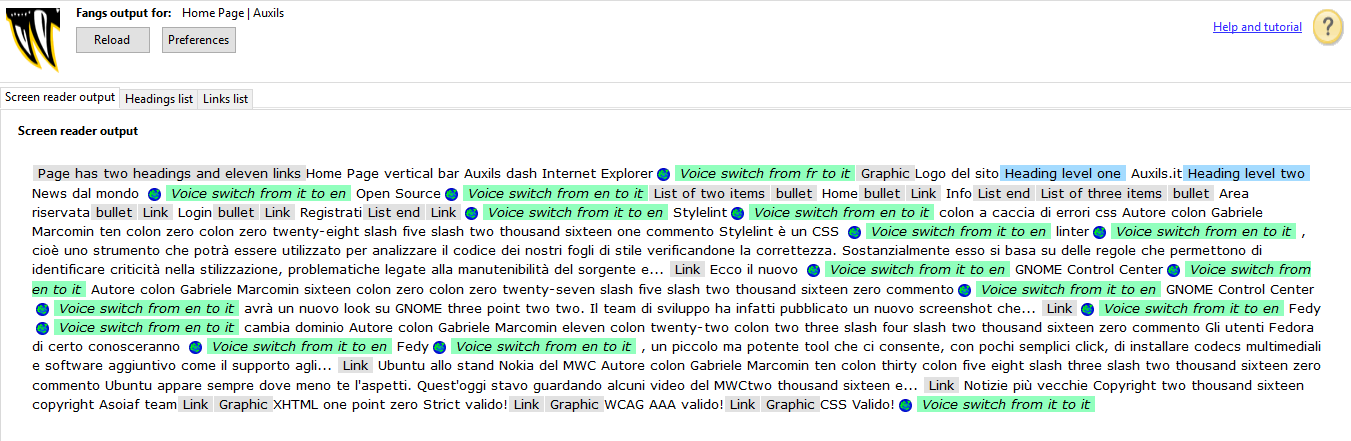
\includegraphics[width=0.8\textwidth]{images/fangs.png}
  \caption{Home visualizzata con Fangs}
\end{figure}

\begin{figure}[H]
  \centering 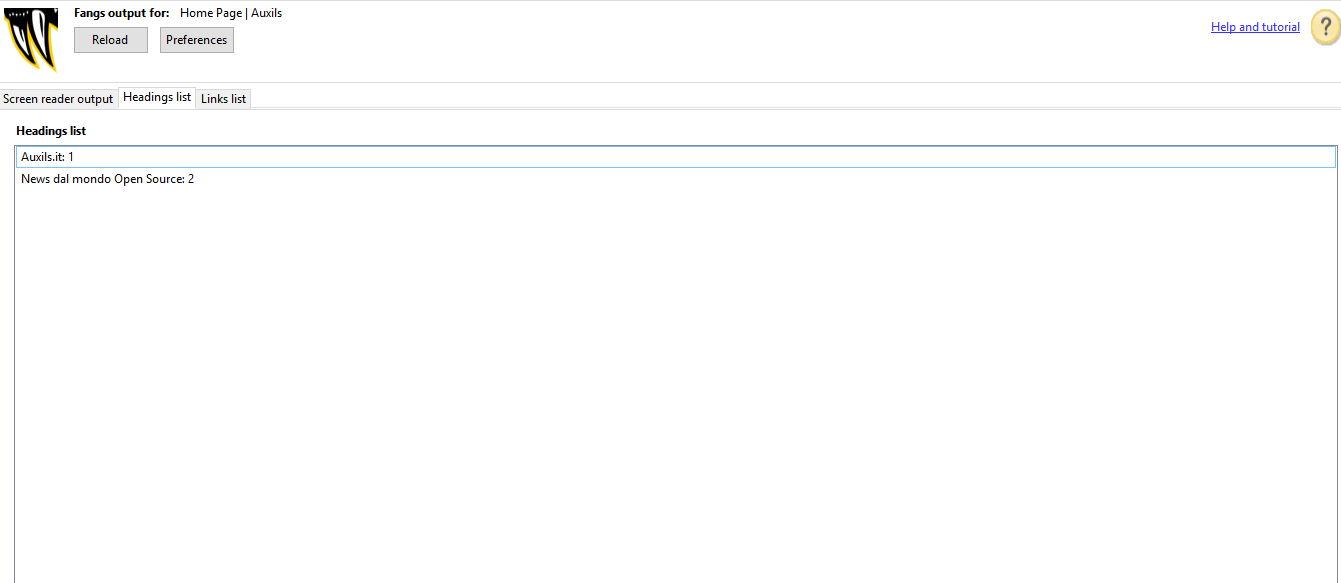
\includegraphics[width=0.8\textwidth]{images/fangsHeader.png}
  \caption{Lista degli header della home visualizzati da Fangs}
\end{figure}
	
\begin{figure}[H]
  \centering 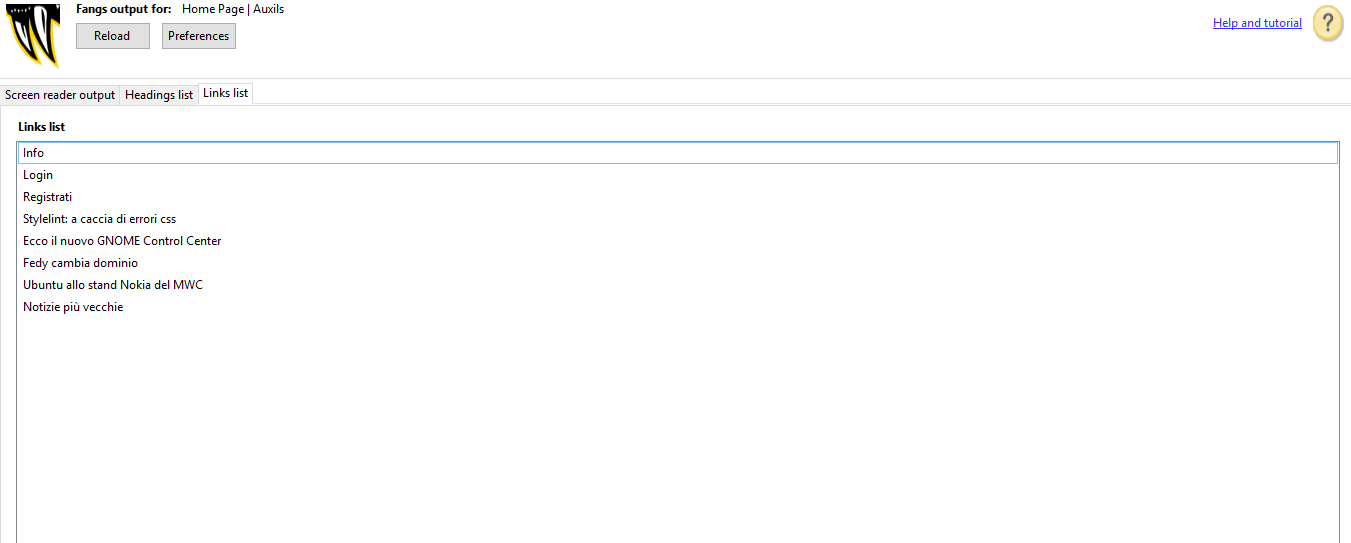
\includegraphics[width=0.8\textwidth]{images/fangsLink.png}
  \caption{Elenco di link contenuti nella home visualizzati da Fangs}
\end{figure}

\subsection{Cecità ai colori}
Al fine di testare che il sito sia accessibile anche da persone che hanno problemi nella corretta visualizzazione dei colori, si è utilizzato ImageJ e l'estensione Vischeck.
Tale estensione permette di visualizzare come viene percepita un'immagine da chi soffre di cecità ai colori. Ogni pagina è stata testata in modo da verificare che sia visualizzabile correttamente con il medesimo grado di contrasto da tutte le tipologie di utenti.

\begin{figure}[H]
		\centering 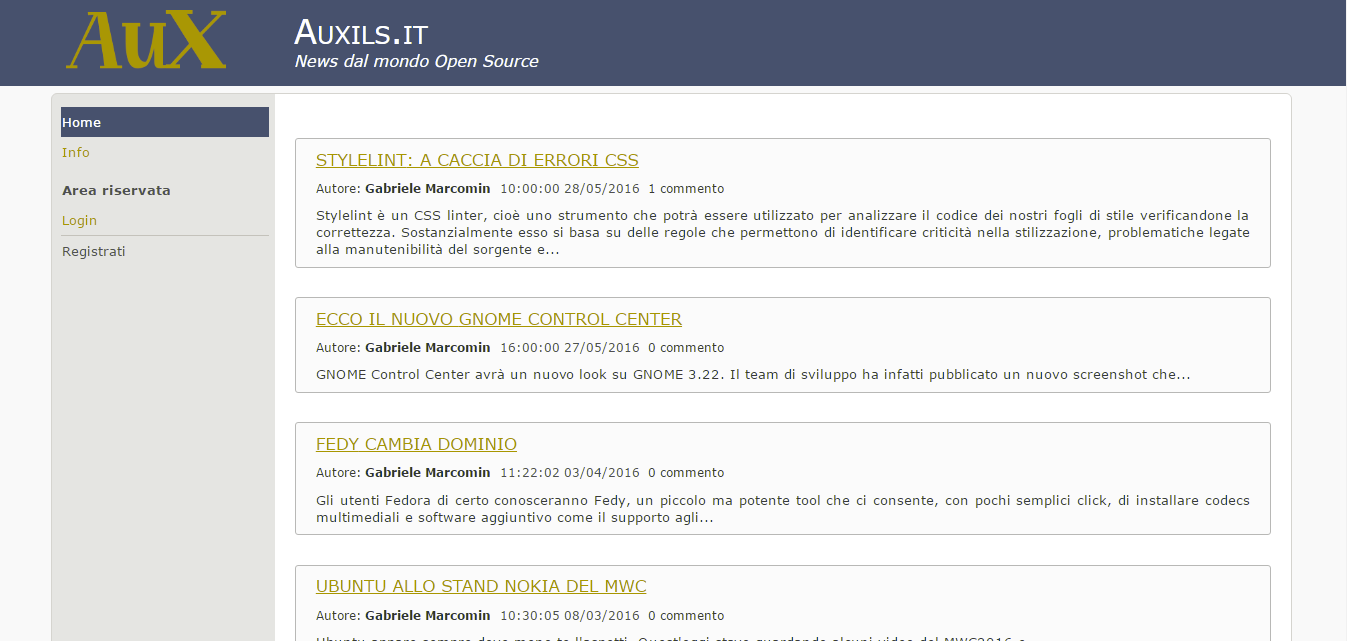
\includegraphics[width=0.9\textwidth]{images/deute.png}
		\caption{Home vista da chi soffre di deuteranopia}
\end{figure}
	
\begin{figure}[H]
		\centering 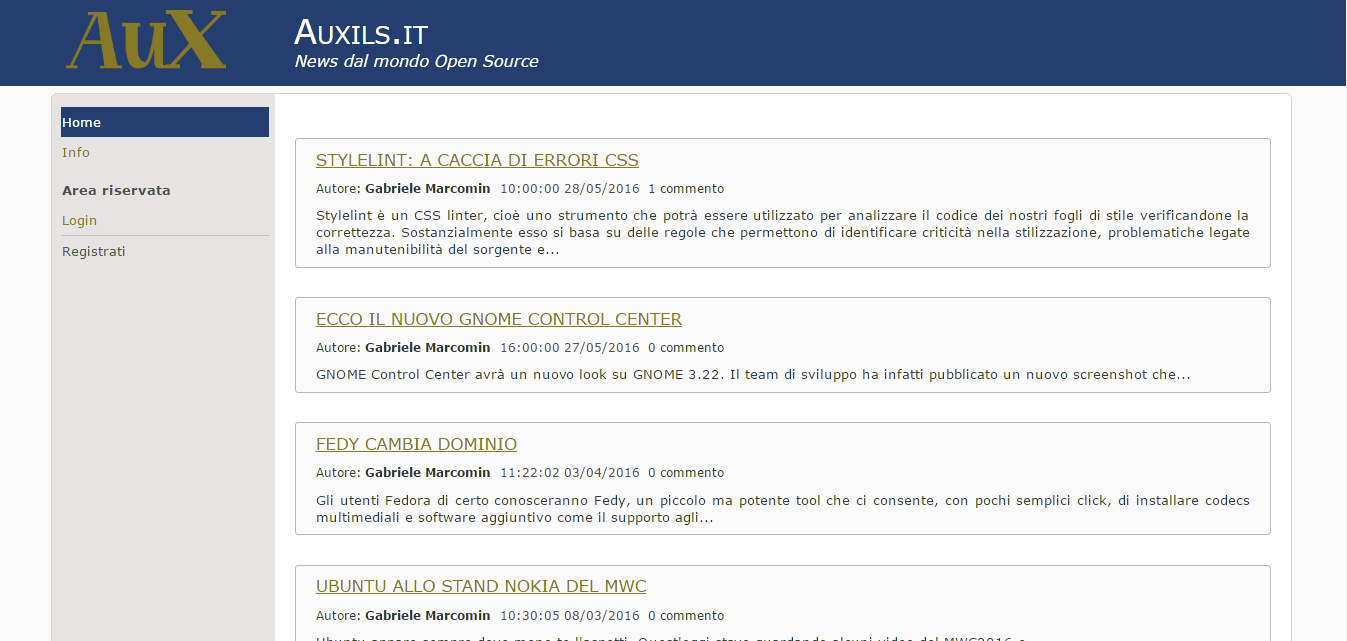
\includegraphics[width=0.9\textwidth]{images/proto.png}
		\caption{Home di pagina vista da chi soffre di protanopia}
\end{figure}
	
\begin{figure}[H]
		\centering 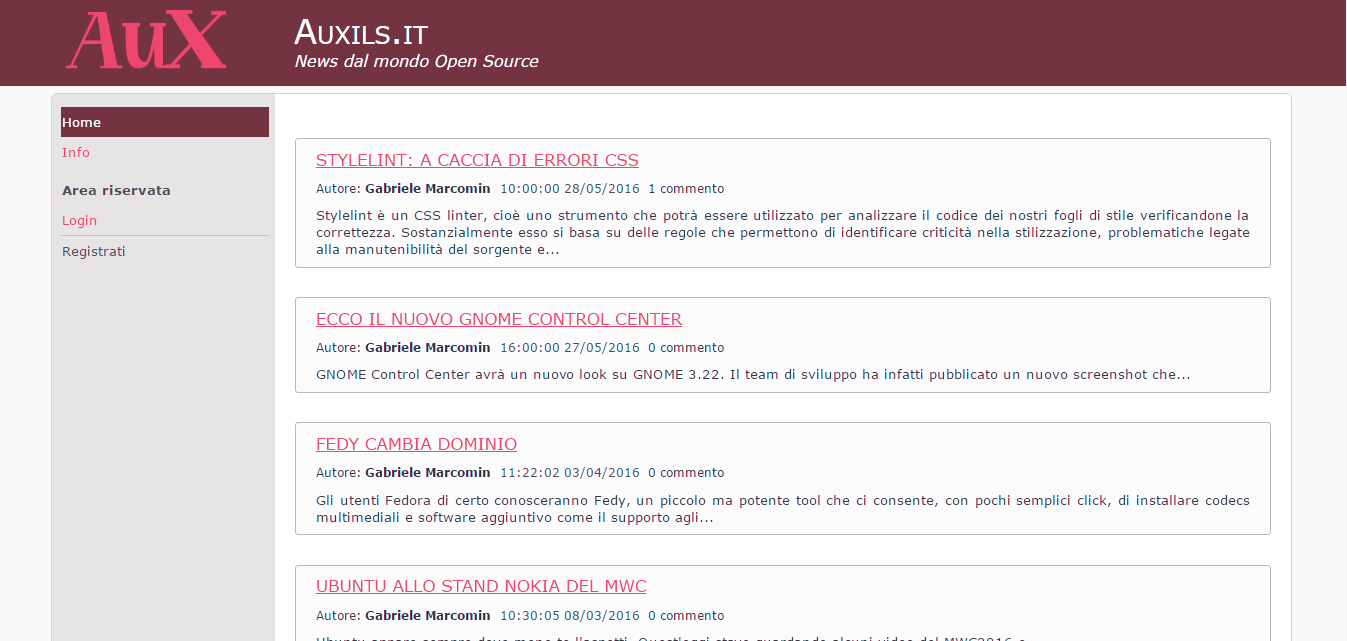
\includegraphics[width=0.9\textwidth]{images/trita.png}
		\caption{Home di pagina vista da chi soffre di tritanopia}
\end{figure}

\subsection{Form}
Durante la realizzazione dei vari form, sono stati tenuti i seguenti accorgimenti al fine di ottenere un buon grado di accessibilità ed usabilità generale:
\begin{itemize}
 \item ad ogni elemento input, di tipo text e textarea, è associata la relativa label con attributo for;
 \item ogni label di ogni campo obbligatorio ha come ultimo carattere il carattere *, per far notare meglio l'obbligatorietà del l'inserimento del campo;
 \item in caso di valori inseriti non validi, gli script Javascript e gli script cgi avvertiranno l'utente con dei messaggi. Come detto in precedenza, in caso di disattivazione di Javascript gli script perl visualizzeranno il medesimo messaggio per lo stesso tipo di errore occorso;
 \item l'utilizzo di fieldset e legend al fine di raggruppare e descrivere un insieme di campi.
\end{itemize}

\subsection{Linee guida per il testo}

Le regole per testi alternativi alle immagini sono le seguenti:
\begin{itemize}
 \item il testo deve presentare il contenuto e la funzione dell'immagine;
 \item alt ed eventuali descrizioni sotto l'immagine non devono presentare lo stesso contenuto;
 \item il testo degli alt e delle eventuali descrizioni deve essere breve e conciso;
 \item alt ed eventuali descrizioni non devono iniziare con "immagine di.." o simili.
\end{itemize}

Per tabelle le regole usate sono le seguenti:
\begin{itemize}
 \item l'utilizzo di caption per dotare la tabella di un titolo;
 \item l'utilizzo di summary per dotare una descrizione del contenuto alla tabella, al fine di aiutare gli utenti non vedenti a comprendere velocemente il contenuto della tabella senza doverlo vedere tutto per capirlo;
 \item l'utilizzo di th per fornire contesto alle varie celle della tabella.
\end{itemize}

\subsection{Tastiera}
Condizione necessaria, ma non sufficiente, ad un sito per essere accessibile è che possa essere navigato utilizzando solamente la tastiera. Ogni pagina è stata testata al fine di verificare che la condizione di navigabilità via tastiera sia sempre rispettata.\\
Non sono stati utilizzati tabindex per i link della barra di navigazione in quanto il sito possiede un flusso semplice e lineare.

\subsection{Total Validator}
Total Validator è una applicazione che permette di verificare l'accessibilità di una pagina web secondo alcuni parametri.\\
Le impostazioni scelte per Total Validator sono state le più stringenti, richiedendo un'accessibilità aderente allo standard WCAG 2.0 AAA.\\
L'esito delle verifiche è stato positivo allo standard, in quanto non sono stati rilevati errors o warnings.
\section{Compatibilità con i browser}
Per confermare la compatibilità e il medesimo grado di accessibilità, sono state testati più browser in modo da accertarsi della bontà di Auxils.it. Il sito mantiene lo stesso grado di accessibilità con tutti i browser testati, tutti gli script Javascript funzionano appieno su tutti i browser testati e le differenze sono presenti in minima parte in Internet Explorer solamente nella presentezione.\\
\subsection{Internet Explorer 6}
Vista la penuria di browser simulati dalla versione di prova di BrowserStack, ho dovuto affidarmi per la simulazione di Internet Explorer 6 ad IETester, un programma open source che permette di simulare Internet Explorer dalla versione 5.5 alla versione 11. Il problema di questa applicazione è che simula con un ottimo livello di stabilità solamente Internet Explorer 6, avendo ancora problemi con le altre versioni.\\
\begin{figure}[H]
  \centering 
\includegraphics[width=0.6\textwidth]{images/homeie6.png}
  \caption{Home visualizzata simulando Internet Explorer 6}
\end{figure}
L'utilizzo di un esiguo numero di costrutti di CSS 3 ha permesso di avere da subito un sito portabile, accattivante ed accessibile allo stesso tempo, anche da browser non al passo coi tempi. Sono state usate comunque soluzioni utili ad aumentare la compatibilità con più browser possibili, mantenendo il medesimo aspetto grafico e grado di accessibilità.\\
Non sono state supportate le seguenti caratteristiche:
\begin{itemize}
  \item i bordi arrotondati non vengono visualizzati;
  \item il foglio di stile per risoluzioni inferiori a 480px non viene attivato;
  \item il bordo inferiore dell'ultimo elemento contenuti nella barra di navigazione viene comunque visualizzato;
  \item i pixel trasparenti del logo vengono sostituiti con pixel di colore bianco.
\end{itemize}
\begin{figure}[H]
  \centering 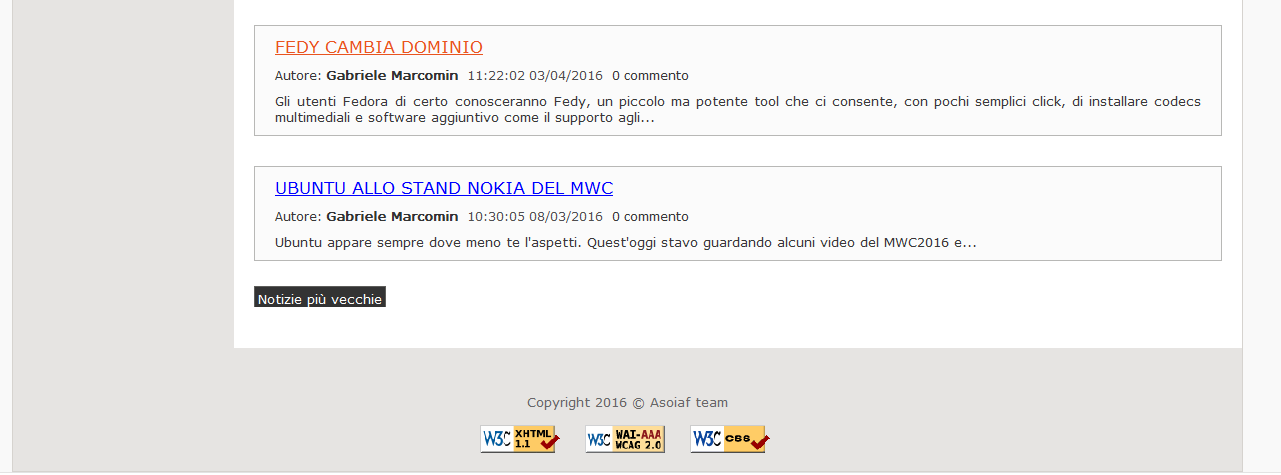
\includegraphics[width=0.6\textwidth]{images/homeie62.png}
  \caption{Footer visualizzato simulando Internet Explorer 6}
\end{figure}
\subsection{Altri browser}
Il sito è stato testato sulle ultime versioni di Microsoft Edge, Chrome, Firefox, Safari e su Internet Explorer 11 grazie a BrowserStack; il test ha potuto dimostrare la piena compatibilità di Auxils.it con i browser precedentemente elencati.
\end{document}
